\documentclass[10pt,conference]{IEEEtran}
\usepackage[utf8]{inputenc}
\usepackage[T1]{fontenc}
\usepackage[spanish,es-tabla]{babel}
\usepackage{amsmath,amssymb}
\usepackage{graphicx}
\usepackage{booktabs}
\usepackage{siunitx}
\usepackage{tikz}
\usetikzlibrary{arrows.meta,positioning,fit,backgrounds,shapes.geometric}
\usepackage[
  backend=biber,
  style=ieee,
  sorting=none
]{biblatex}
\addbibresource{references.bib}
\usepackage{hyperref}
\usepackage{url}
\usepackage{caption}
\usepackage{float}

\sisetup{
  output-decimal-marker = {,},
  per-mode = symbol
}

\title{Análisis de Rendimiento Paralelo aplicado al Proyecto Fin de Curso:\\
Del ordenamiento y \emph{Top-N} distribuido en PySpark a la propuesta de\\
integración en el Sistema de Control de Laboratorios Informáticos (SCLI)}

\author{
\IEEEauthorblockN{Iván Andrés Villamarín Cuenca}
\IEEEauthorblockA{Facultad de Ciencias de la Computación --- UTEQ}
}

\begin{document}
\shorthandoff{<>}


\begin{titlepage}
\onecolumn
\centering
\vspace*{1cm}
{\large UNIVERSIDAD TÉCNICA ESTATAL DE QUEVEDO}\\[2mm]
{\normalsize Facultad de Ciencias de la Computación}\\
{\normalsize Carrera de Ingeniería de Software}\\[10mm]

{\Large\bfseries Código de actividad: TA-IND-04}\\[2mm]
{\normalsize Trabajo Autónomo Individual --- Informe Técnico}\\[10mm]

\rule{0.9\linewidth}{0.4pt}\\[4mm]
{\LARGE\bfseries Análisis de Rendimiento Paralelo aplicado al Proyecto Fin de Curso}\\[3mm]
{\large Del ordenamiento y \emph{Top-N} distribuido en PySpark a la propuesta de integración\\ en el Sistema de Control de Laboratorios Informáticos (SCLI)}\\[4mm]
\rule{0.9\linewidth}{0.4pt}\\[12mm]

\begin{tabular}{@{}rl@{}}
\textbf{Asignatura:} & Aplicaciones Distribuidas (ISR-701) \\[1mm]
\textbf{Unidad:} & Unidad 4 --- Cómputo Paralelo y Distribuido \\[1mm]
\textbf{Práctica de origen:} & GA-SUM-05 / PE-U4 --- Procesamiento Distribuido con Apache Spark \\[1mm]
\textbf{Estudiante:} & Iván Andrés Villamarín Cuenca \\[1mm]
\textbf{Equipo de PE-U4:} & Equipo C --- Freddy Farinango, Jeremy Gaibor, Iván Villamarín \\[1mm]
\textbf{PFC de referencia:} & SCLI --- Sistema de Control de Laboratorios Informáticos \\[1mm]
\textbf{Transformación foco:} & T5 --- Ordenamiento y Top-20 \\[1mm]
\textbf{Repositorio (este informe):} & \url{https://github.com/iavillamarin98-pred/ta-ind-04-villamarin} \\[1mm]
\textbf{Repositorio de origen (PE-U4):} & \url{https://github.com/ffarinangog2/pe-u4-spark-equipo-c} \\[1mm]
\textbf{Commit de los datos base:} & \texttt{3a0ae757b6f8288bf095905e286bca75d8026a36} \\[1mm]
\textbf{Docente:} & Gleiston C. Guerrero-Ulloa, M.Sc. \\[1mm]
\textbf{Período académico:} & 2026--2027 PPA \\[1mm]
\textbf{Fecha:} & \today \\
\end{tabular}

\vfill
\end{titlepage}
\twocolumn


\maketitle

\begin{abstract}
Este informe analiza de forma individual los resultados de \textit{speedup} obtenidos en la práctica grupal GA-SUM-05/PE-U4 --- \textit{Procesamiento Distribuido con Apache Spark} --- para la transformación T5 (ordenamiento global y selección de las 20 solicitudes de mayor demanda) sobre un conjunto sintético de 500\,000 solicitudes de reserva de laboratorios, ejecutada en pandas y en PySpark 3.5.0 sobre un clúster Spark Standalone real de hasta cuatro \textit{executors}. A diferencia de otras transformaciones del equipo, T5 cuenta con mediciones propias de escalado en $N=1,2,4$ \textit{executors}, lo que permite un análisis cuantitativo completo frente a la Ley de Amdahl y la métrica de Karp-Flatt. Se determina que, a diferencia de las transformaciones más ligeras del \textit{pipeline}, el umbral de rentabilidad de T5 ya se cruza al volumen actual, y se propone un punto concreto de integración de un servicio de generación de rankings en la arquitectura de microservicios del Sistema de Control de Laboratorios Informáticos (SCLI).
\end{abstract}

\section{Introducción y contexto}
\label{sec:intro}

El presente documento constituye la entrega individual TA-IND-04 de la asignatura Aplicaciones Distribuidas (ISR-701), Unidad 4 -- Cómputo Paralelo y Distribuido. Su objetivo es explotar intelectualmente, de forma individual, los datos experimentales producidos en equipo durante la práctica \textbf{GA-SUM-05/PE-U4 --- Procesamiento Distribuido con Apache Spark: comprobación experimental de la Ley de Amdahl}, en la cual se compararon cinco transformaciones (T1--T5) sobre un mismo conjunto de datos, ejecutadas alternativamente con pandas (motor secuencial de referencia) y con PySpark (motor distribuido) sobre un clúster Spark Standalone real.

El experimento de origen se realizó sobre un conjunto sintético y reproducible de 500\,000 solicitudes de reserva de laboratorios y 40 laboratorios, relacionados 1:N mediante \texttt{laboratorio\_id}, generado con semilla fija \texttt{20260804} para el dominio FUVV -- Sistema de Control de Laboratorios Informáticos. Se utilizan datos sintéticos porque no existen 500\,000 registros operacionales públicos adecuados para el volumen exigido y porque así se evita el uso de información personal real de estudiantes o docentes.

Los datos base de este informe proceden del repositorio del equipo:
\begin{itemize}
  \item \textbf{Repositorio PE-U4:} \url{https://github.com/ffarinangog2/pe-u4-spark-equipo-c}
  \item \textbf{Commit exacto:} {\small\texttt{3a0ae757\-b6f8288b\-f0959059\-05e286bc\-a75d8026a36}} (rama \texttt{main})
  \item \textbf{Archivo fuente:} \texttt{resultados/tiempos\_resumen.csv} y \texttt{resultados/tiempos\_crudos.csv}
\end{itemize}

La transformación declarada como foco individual de este análisis es \textbf{T5 -- ordenamiento global y selección \textit{Top-20}}: las solicitudes se ordenan de forma estable por número de participantes y duración descendentes, con fecha e identificador como criterios de desempate ascendentes, y se seleccionan las 20 de mayor demanda. Es, junto con T3, una de las transformaciones para las que el equipo generó mediciones escaladas propias en $N=1,2,4$ \textit{executors}, condición indispensable para el análisis cuantitativo de escalabilidad que exige este instrumento. El dominio del PFC de referencia es el Sistema de Control de Laboratorios Informáticos (SCLI), un sistema de microservicios (Spring Boot, CockroachDB, Docker Compose) actualmente en desarrollo para automatizar la gestión de usuarios, laboratorios, reservas y solicitudes de la institución.

\section{Análisis propio de los resultados de \textit{speedup}}
\label{sec:analisis}
\subsection{Datos base y trazabilidad}

La Tabla~\ref{tab:datos} reproduce, con los valores exactos tomados del commit declarado, las medianas de cinco repeticiones para las cinco transformaciones evaluadas por el equipo, junto con el escalado de T5 en $N=1,2,4$ \textit{executors}. La ejecución PySpark se realizó sobre Spark Standalone (\texttt{spark://127.0.0.1:7077}), PySpark 3.5.0, con un núcleo y \SI{512}{\mebi\byte} de memoria por \textit{executor}, sesión independiente creada y destruida para cada configuración de $N$ (sin \textit{caching} entre configuraciones), y con \texttt{spark.sql.shuffle.partitions} y \texttt{spark.default.parallelism} fijados explícitamente en $N$ --- condición declarada en la configuración del equipo (verificada mediante \texttt{StatusTracker} antes de cada medición) que resulta determinante para el diagnóstico de la Sección~\ref{sec:diagnostico}.

\begin{table}[H]
\centering
\caption{Tiempos medianos (5 repeticiones) por transformación y configuración. Fuente: \texttt{resultados/tiempos\_resumen.csv}, commit \texttt{3a0ae757}.}
\label{tab:datos}
\begin{tabular}{@{}llS[table-format=1.4]@{}}
\toprule
\textbf{Transf.} & \textbf{Motor / config.} & {\textbf{Mediana (s)}} \\
\midrule
T1 & pandas               & 0.2119 \\
T1 & PySpark, $N{=}4$     & 0.3457 \\
T2 & pandas               & 0.1171 \\
T2 & PySpark, $N{=}4$     & 0.6875 \\
T3 & pandas               & 0.2889 \\
T3 & PySpark, $N{=}4$     & 0.8657 \\
T4 & pandas               & 2.2659 \\
T4 & PySpark, $N{=}4$     & 1.8100 \\
T5 & pandas               & 1.5252 \\
T5 & PySpark, $N{=}1$     & 1.5632 \\
T5 & PySpark, $N{=}2$     & 1.1733 \\
T5 & PySpark, $N{=}4$     & 1.3565 \\
\bottomrule
\end{tabular}
\end{table}

De las cinco transformaciones, pandas superó a PySpark en T1, T2 y T3, mientras que PySpark fue más rápido en T4 (columna derivada, con cómputo por fila más costoso) y \textbf{T5} (ordenamiento total y \textit{top-N}), con un \textit{speedup} cruzado $S_{\text{pandas/PySpark}} = T_{\text{pandas}}/T_{\text{PySpark}}(N{=}4) = 1{,}5252/1{,}3565 = 1{,}1244$. Este patrón es consistente con la literatura: PySpark amortiza mejor su sobrecarga de planificación cuando el costo de cómputo por registro es alto --- el ordenamiento global de 500\,000 filas antes de recortar el \textit{top-20} es, junto con T4, la operación más costosa del \textit{pipeline} en pandas (\SI{1.5252}{\second}) --- mientras que en operaciones ligeras (filtrado, agrupación simple, \textit{join} sencillo) esa sobrecarga fija domina el tiempo total \cite{zaharia2016spark}.

\subsection{Contraste experimental frente a la predicción de Amdahl}

A diferencia del \textit{speedup} cruzado pandas/PySpark reportado arriba, el análisis de escalabilidad exige el \textit{speedup} \textbf{interno} de PySpark, tomando como referencia $N=1$:
\begin{equation}
S(N) = \frac{T_{\text{PySpark}}(N{=}1)}{T_{\text{PySpark}}(N)}, \qquad N \in \{1,2,4\}.
\label{eq:speedup_exp}
\end{equation}
Estas son magnitudes distintas y no deben confundirse: $S_{\text{pandas/PySpark}}$ compara dos motores a igual $N$, mientras que $S(N)$ de la Ec.~\eqref{eq:speedup_exp} mide la ganancia de paralelizar \emph{dentro} de PySpark al variar $N$, que es la que exige la Ley de Amdahl.

Con los tiempos de la Tabla~\ref{tab:datos}: $S(1)=1{,}0000$, $S(2)=1{,}3324$, $S(4)=1{,}1524$. El resultado es, igual que en la transformación T3 del equipo, \textbf{no monótono}: el \textit{speedup} en $N=4$ es menor que en $N=2$, es decir, añadir dos \textit{executors} adicionales \emph{empeoró} el rendimiento respecto de $N=2$. Este comportamiento por sí solo ya adelanta que el modelo de Amdahl, que asume una fracción paralelizable constante y sobrecarga nula \cite{hillmarty2008}, no podrá ajustar simultáneamente los tres puntos.

Siguiendo la Ec.~\eqref{eq:amdahl}, formulación original de la Ley de Amdahl \cite{amdahl1967}, se estimó la fracción paralelizable $p$ mediante un ajuste de un único punto anclado en $N=4$ (la configuración con mayor paralelismo disponible), despejando $p$ de $1/S(4) = (1-p) + p/4$:
\[
p = \frac{1 - 1/S(4)}{0{,}75} = 0{,}1764.
\]

Con este $p$, la Ec.~\eqref{eq:amdahl} predice $S_{\text{teo}}(2)=1{,}0967$ y, por construcción, $S_{\text{teo}}(4)=1{,}1524$ (coincide exactamente con el punto de anclaje). El límite máximo teórico es $S_{\max}=1/(1-p)=1{,}2141$: incluso con \textit{executors} infinitos, T5 nunca podría acelerarse más de un \SI{21.4}{\percent} respecto de un solo \textit{executor} --- una fracción paralelizable mucho más pequeña que la de T3 (donde $p\approx0{,}4855$), coherente con que un ordenamiento global (\textit{sort}) es intrínsecamente más dependiente de coordinación entre particiones que un \textit{join}.

La desviación relativa (Sección 4.1 de la guía) se calcula como
\[
\Delta = \frac{S_{\text{med}} - S_{\text{teo}}}{S_{\text{teo}}} \times 100\%.
\]

En $N=4$, $\Delta=0{,}0\%$ por construcción del ajuste. En $N=2$, sin embargo, $\Delta = +21{,}5\%$: el \textit{speedup} medido \textbf{supera} la predicción teórica, un caso de \textit{speedup superlineal} local que la guía no enumera entre sus tres respuestas típicas (coincidencia, déficit, o $S<1$) pero que es perfectamente consistente con el marco de Amdahl si se explica el mecanismo.

\textbf{¿Coinciden los resultados con la predicción de Amdahl?} No de forma uniforme, y la razón tiene dos componentes identificables. Primero, el ajuste de $p$ con un solo punto ($N=4$) no es un ajuste por mínimos cuadrados sobre las tres observaciones; al anclarse en el extremo de mayor $N$, el modelo resultante no está obligado a explicar el comportamiento en $N=2$, y de hecho no lo hace. Segundo, y más relevante en términos de sistema real: en $N=2$ el volumen de trabajo por \textit{executor} es el doble que en $N=4$ (250\,000 vs.\ 125\,000 registros), lo que favorece una mejor razón entre trabajo útil y sobrecarga fija de \textit{shuffle} y planificación por tarea; en $N=4$ esa misma sobrecarga fija se paga cuatro veces por una fracción de datos cada vez menor por \textit{executor}, un efecto de rendimientos decrecientes que Amdahl, al asumir sobrecarga nula, no puede capturar \cite{hillmarty2008}. Esto también es coherente con el argumento de Gustafson de que el comportamiento del \textit{speedup} depende fuertemente de cómo escala el trabajo por unidad de procesamiento, no solo del número de unidades \cite{gustafson1988}.

\subsection{Figura propia}

La Fig.~\ref{fig:speedup} (elaboración propia, generada con el script \texttt{figuras/generar\_fig\_speedup.py} incluido en este repositorio) superpone la curva teórica de Amdahl ajustada en $N=4$ con los tres puntos experimentales de T5. La brecha visual entre la curva y el punto $N=2$ hace explícita la superlinealidad discutida arriba, mientras que en $N=4$ la curva y el punto coinciden por construcción del ajuste. Nótese la escala vertical mucho más comprimida que la de una transformación con mayor fracción paralelizable: el margen de mejora total de T5 mediante paralelismo puro es, según $S_{\max}$, inferior al \SI{22}{\percent}.

\begin{figure}[H]
\centering
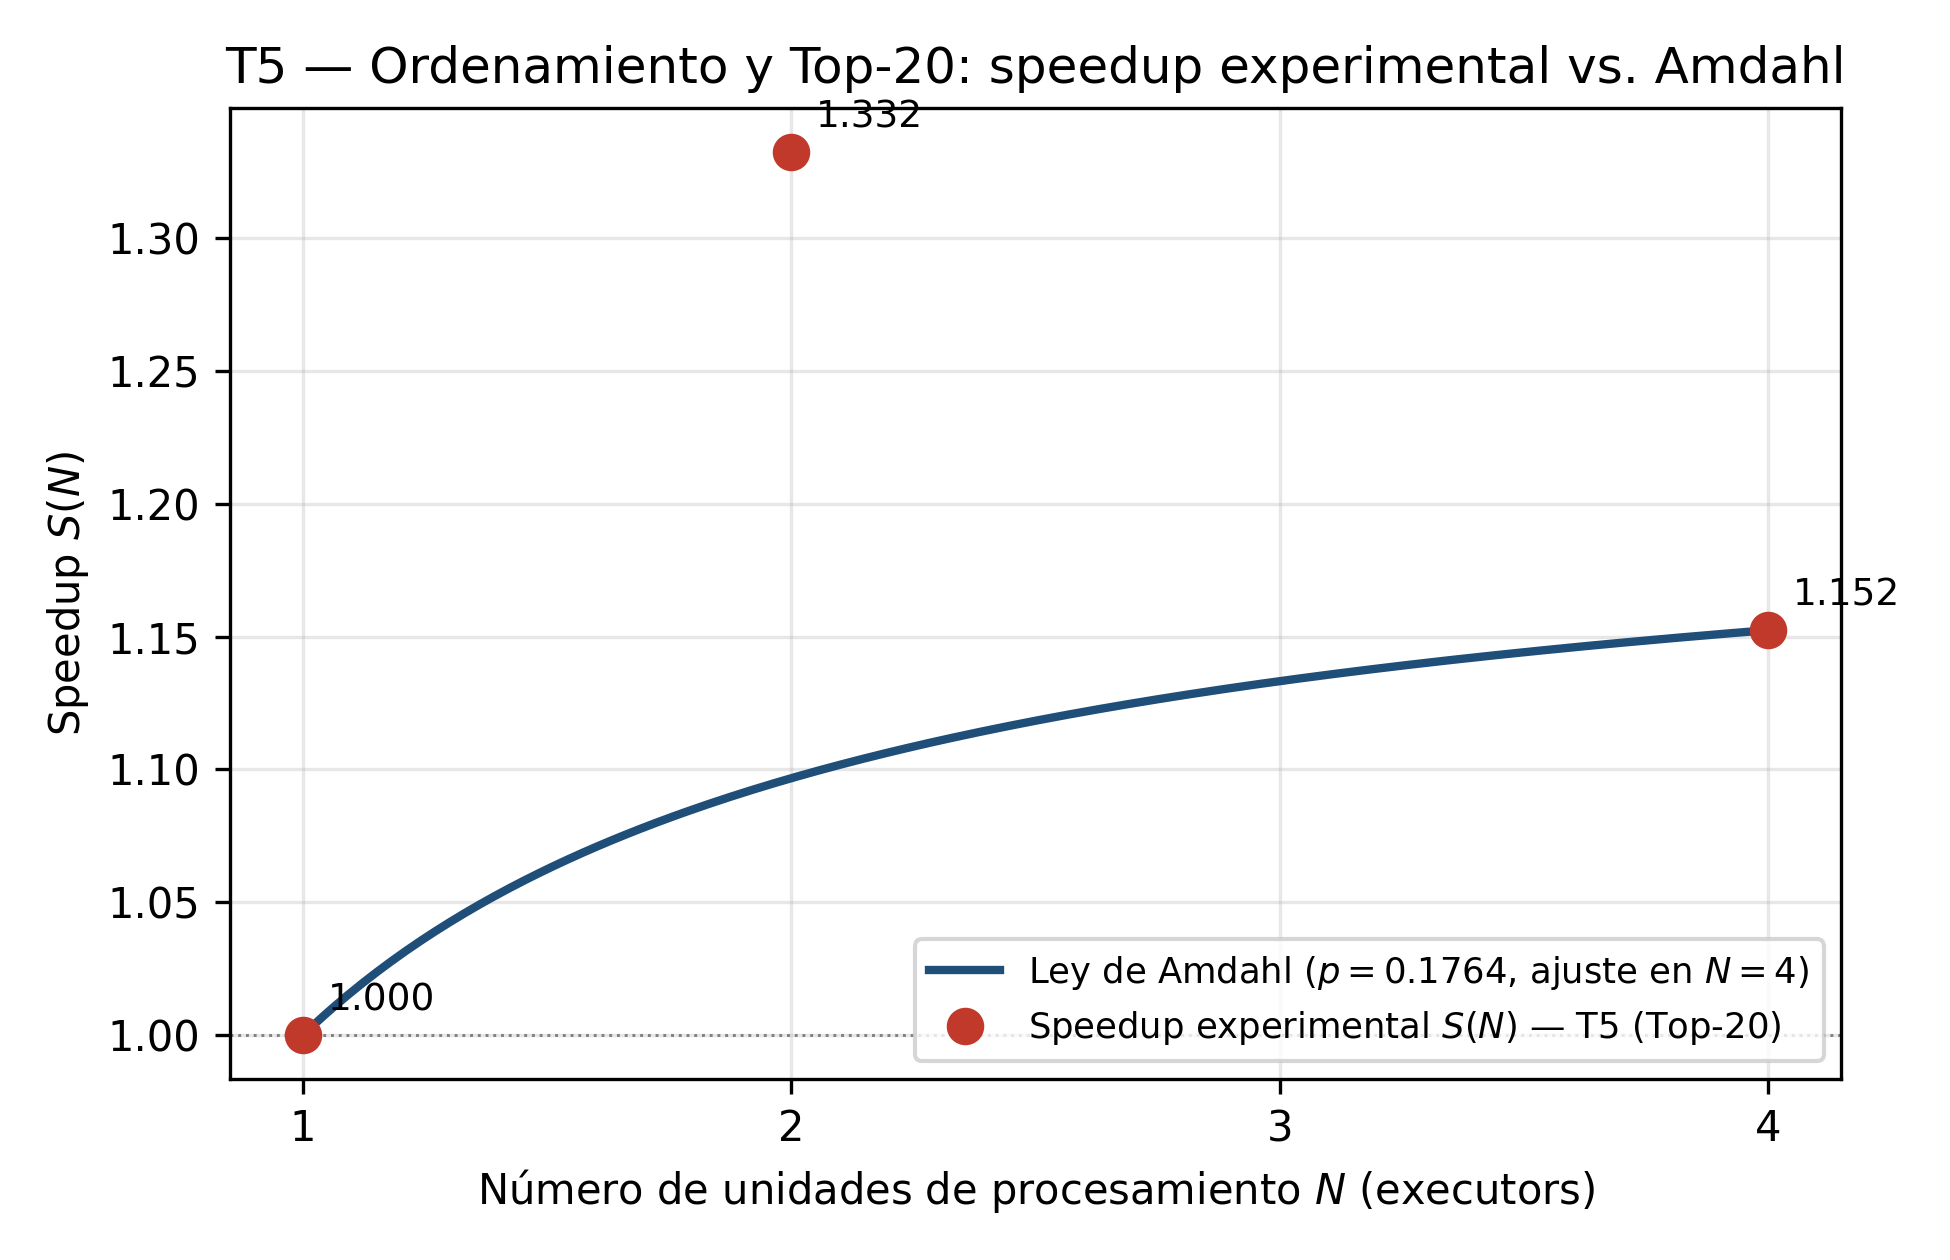
\includegraphics[width=0.95\linewidth]{../figuras/fig_speedup.png}
\caption{Speedup experimental $S(N)$ de T5 (ordenamiento y \textit{Top-20}) frente a la curva teórica de Amdahl ajustada en $N=4$ ($p=0{,}1764$). Elaboración propia a partir de \texttt{tiempos\_resumen.csv}, commit \texttt{3a0ae757}.}
\label{fig:speedup}
\end{figure}

\section{Diagnóstico de la fracción no escalable}
\label{sec:diagnostico}

\subsection{Métrica de Karp-Flatt y su tendencia}

La fracción serial experimental $e$ se calculó con la Ec.~\eqref{eq:karpflatt} para $N=2$ y $N=4$, usando los mismos valores de $S(N)$ obtenidos en la Sección~\ref{sec:analisis}:
\[
e(2) = \frac{1/S(2) - 1/2}{1 - 1/2} = 0{,}5010, \qquad
e(4) = \frac{1/S(4) - 1/4}{1 - 1/4} = 0{,}8236.
\]

La tendencia es inequívoca y creciente: $e$ pasa de \SI{50.1}{\percent} a \SI{82.4}{\percent} entre $N=2$ y $N=4$. Según el criterio de interpretación de Karp y Flatt \cite{karpflatt1990}, una fracción serial que permanece aproximadamente constante al variar $N$ indica un límite algorítmico de paralelismo; una fracción serial que \emph{crece} con $N$, como en este caso, indica que la pérdida de eficiencia proviene predominantemente de la \textbf{sobrecarga creciente del motor}, no solo del algoritmo. A diferencia de T3, sin embargo, aquí el punto de partida ya es alto ($e(2)=0{,}5010$): más de la mitad del tiempo de T5 con dos \textit{executors} ya es no paralelizable, coherente con el bajo $p=0{,}1764$ estimado en la Sección~\ref{sec:analisis} --- el ordenamiento global tiene, por su propia naturaleza algorítmica, una fracción serial estructuralmente mayor que un \textit{join}.

\subsection{Atribución de la sobrecarga a mecanismos concretos}

Se identifican tres mecanismos concretos, coherentes con la arquitectura de ejecución de Spark \cite{zaharia2012rdd,zaharia2016spark} y con la configuración efectivamente empleada por el equipo (Tabla de configuración del repositorio de origen), que explican tanto el nivel alto de $e$ como su crecimiento entre $N=2$ y $N=4$ para un ordenamiento global de 500\,000 filas:

\begin{itemize}
  \item \textbf{\textit{Range partitioning} para el orden total.} A diferencia de una transformación estrecha, un \texttt{orderBy} global en Spark exige primero muestrear la distribución de las claves de ordenamiento (participantes y duración) para determinar los límites de rango de cada partición, y luego redistribuir --- vía \textit{shuffle} --- cada fila a la partición cuyo rango le corresponde, de modo que el orden final quede correcto entre particiones. Con \texttt{spark.sql.shuffle.partitions}\,$=N$ fijado por el equipo, al pasar de $N=2$ a $N=4$ este muestreo y la redistribución se fragmentan en el doble de particiones, cada una más pequeña, sin que el costo fijo de calcular los límites de rango y coordinar la redistribución se reduzca proporcionalmente --- el mecanismo de rendimientos decrecientes que Amdahl, al asumir sobrecarga nula, no puede capturar \cite{hillmarty2008}.
  \item \textbf{Recolección final del \textit{Top-20} en el \textit{driver}.} A diferencia de T3 (cuyo resultado son las 500\,000 filas del \textit{join}), T5 termina con una acción \texttt{limit(20)} que exige fusionar los resultados parcialmente ordenados de cada partición en un único orden global de solo 20 filas en el \textit{driver}. Esa fusión final es inherentemente serial --- es, de hecho, la porción de la fracción serial algorítmica genuina de T5, distinta de la sobrecarga del motor --- y explica por qué $p$ es estructuralmente bajo para esta transformación incluso antes de considerar la sobrecarga de \textit{shuffle}.
  \item \textbf{Contención de recursos entre \textit{executors} concurrentes en una sola máquina física.} Cada \textit{executor} se configuró con un solo núcleo y \SI{512}{\mebi\byte} de memoria, ejecutado como proceso JVM independiente sobre el mismo \textit{host} físico (Spark Standalone local). Con $N=4$ \textit{executors} concurrentes compitiendo por la misma CPU, memoria y E/S de disco de una sola máquina, la presión de memoria durante el \textit{shuffle} de ordenamiento se agrava de forma no lineal respecto de $N=2$, un efecto que un clúster de nodos físicos separados no presentaría con la misma magnitud.
\end{itemize}

\textbf{¿Qué parte de la no escalabilidad es atribuible al algoritmo y qué parte al motor?} A diferencia de T3, en T5 ambas partes son sustanciales: la fusión final del \textit{Top-20} en el \textit{driver} es una fracción serial \emph{algorítmica} genuina (no desaparece aunque el motor no tuviera sobrecarga alguna), mientras que el crecimiento de $e$ entre $N=2$ y $N=4$ --- que un algoritmo de ordenamiento intrínsecamente no escalable no explicaría por sí solo, porque su complejidad teórica no cambia con $N$ --- es atribuible a la sobrecarga creciente del \textit{range partitioning} y del \textit{shuffle} del motor.

\section{Propuesta de integración al PFC}
\label{sec:propuesta}

\subsection{Caso de uso y arquitectura de integración}

El PFC de referencia es SCLI, un sistema de microservicios (Java 21, Spring Boot 4.1.0, Spring Cloud Gateway, CockroachDB, Docker Compose) que gestiona usuarios, laboratorios, académico y reservas/solicitudes de laboratorios informáticos institucionales. Actualmente el servicio \texttt{reservas-solicitudes-service} (puerto 8084, base \texttt{reservas\_db}) está en fase de integración al \textit{gateway}.

El caso de uso concreto propuesto es la \textbf{generación periódica del ranking de laboratorios y solicitudes de mayor demanda}, aplicación directa de T5: ordenar el historial acumulado de \texttt{solicitudes\_reserva} por número de participantes y duración, con fecha e identificador como desempate, y publicar el \textit{Top-N} de mayor demanda para apoyar la asignación de franjas horarias, la priorización de solicitudes en \texttt{SOLICITUD\_APROBAR} y la planificación de ampliación de capacidad. Se trata de un proceso por \textbf{lotes (batch)}, no en flujo, porque el ranking no necesita recalcularse ante cada solicitud individual, y ejecutarlo con una periodicidad fija (p.\ ej., diaria o al cierre de cada período de matrícula) es suficiente para las decisiones de negocio que soporta.

La Fig.~\ref{fig:arquitectura} muestra el punto de inserción propuesto: un nuevo componente \texttt{ranking-batch-service} que se suscribe periódicamente a una réplica de solo lectura de \texttt{reservas\_db} (evitando carga adicional sobre la base transaccional), ejecuta el ordenamiento distribuido y publica el \textit{Top-N} resultante de vuelta en \texttt{reservas\_db} para que \texttt{reservas-solicitudes-service} lo consuma a través del \textit{gateway} ya existente en \texttt{:9090}.

\begin{figure}[H]
\centering
\begin{tikzpicture}[
  node distance=9mm and 6mm,
  box/.style={draw, rounded corners, minimum width=2.5cm, minimum height=0.8cm, align=center, font=\scriptsize},
  db/.style={draw, cylinder, shape border rotate=90, minimum height=0.9cm, minimum width=1.3cm, aspect=0.2, align=center, font=\tiny, inner sep=1pt},
  arr/.style={-{Latex[length=2mm]}, thick}
]
  \node[box, fill=blue!8] (gw) {API Gateway\\ \texttt{:9090}};
  \node[box, below=of gw, fill=gray!10] (res) {reservas-\\solicitudes-service\\ \texttt{:8084}};
  \node[db, below=11mm of res] (resdb) {\texttt{\scriptsize reservas\_db}};
  \node[box, below right=16mm and 2mm of res, fill=orange!15, minimum width=3.2cm, minimum height=1.0cm] (batch) {\textbf{ranking-batch-service}\\ \footnotesize (nuevo --- PySpark, $N{=}2$)};

  \draw[arr] (gw) -- (res);
  \draw[arr] (res) -- (resdb);
  \draw[arr, dashed] (resdb.east) .. controls +(1.2,0) and +(-1.0,0.4) .. (batch.west);
  \draw[arr] (batch.north) .. controls +(-0.3,0.9) and +(1.0,-0.3) .. (resdb.east);

  \matrix[draw, font=\tiny, below=4mm of batch, anchor=north west, row sep=0.5mm] {
    \draw[dashed, arr] (0,0) -- (0.5,0); & \node{réplica de solo lectura}; \\
    \draw[arr] (0,0) -- (0.5,0); & \node{escritura del \textit{Top-N}}; \\
  };
\end{tikzpicture}
\caption{Punto de inserción propuesto de \texttt{ranking-batch-service} en la arquitectura de SCLI. Elaboración propia (TikZ), sobre la topología documentada en el repositorio del PFC.}
\label{fig:arquitectura}
\end{figure}

\subsection{Umbral de rentabilidad y dimensionamiento}

Se estimaron los parámetros de la Ec.~\eqref{eq:umbral} a partir de las mediciones propias de T5. La tasa secuencial $\alpha$ se estimó directamente como $\alpha = T_{\text{pandas}}(n)/n$ con $n=500\,000$:
\[
\alpha = \frac{1{,}52521\ \text{s}}{500\,000} = 3{,}0504\times10^{-6}\ \text{s/registro}.
\]

Los parámetros $\beta$ (sobrecarga fija de la sesión distribuida) y $\gamma$ (costo marginal distribuido) se estimaron por \textbf{mínimos cuadrados ordinarios} sobre las tres mediciones propias de PySpark en T5, tomando $x=n/N$ como variable independiente (válido porque el modelo de la Ec.~\eqref{eq:umbral} depende de $n$ y $N$ exclusivamente a través de esa razón; al mantenerse $n$ fijo en 500\,000 y variar $N\in\{1,2,4\}$, se obtienen tres pares $(x,T_{\text{dist}})$ equivalentes a un barrido de $n/N$):
\[
\beta = 1{,}1615\ \text{s}, \qquad \gamma = 6{,}9545\times10^{-7}\ \text{s/registro}.
\]

Para $N=2$ (la configuración de mejor eficiencia observada, Sección~\ref{sec:formal}), la Ec.~\eqref{eq:umbral} exige $\alpha > \gamma/N$; en efecto $3{,}0504\times10^{-6} > 3{,}4773\times10^{-7}$, por lo que el umbral es válido:
\[
n^{*}_{N=2} = \frac{\beta}{\alpha - \gamma/2} = \frac{1{,}1615}{2{,}7027\times10^{-6}} \approx 429\,751\ \text{registros}.
\]
Para $N=4$, análogamente, $n^{*}_{N=4} \approx 403\,777$ registros.

\textbf{Este es el hallazgo más relevante de la sección}: a diferencia de una transformación ligera como T3 (cuyo umbral, calculado en un análisis paralelo con la misma metodología, ronda los 2,68 millones de registros), \textbf{el umbral de rentabilidad de T5 --- entre 404\,000 y 430\,000 registros según $N$ --- ya está por debajo del volumen actual del experimento (500\,000)}. Es decir, para una operación de ordenamiento global costosa como la generación del ranking de demanda, PySpark \emph{ya} es la opción más barata al volumen que SCLI manejaría desde el primer período de operación, sin necesidad de esperar a que el sistema crezca.

\textbf{Modelo de servicio en la nube.} Dado que SCLI ya despliega mediante Docker Compose, se propone un modelo de \textbf{contenedores gestionados bajo demanda} (p.\ ej., un \textit{job} de Spark en modo \textit{cluster} lanzado por un orquestador como Kubernetes CronJob o, en un proveedor gestionado, AWS Glue/EMR en modo transitorio), creado únicamente durante la ventana de ejecución diaria del ranking y destruido después \cite{dean2015bigdata}. Se recomienda $N=2$ \textit{executors} y no $N=4$: además de tener el umbral de rentabilidad más favorable, $N=2$ ofrece la mejor eficiencia observada (Sección~\ref{sec:formal}), por lo que asignar el doble de recursos en producción desperdiciaría presupuesto sin mejorar --- de hecho, empeorando --- el tiempo de respuesta.

\textbf{Riesgos identificados:} (i) el ajuste de $\beta,\gamma$ se realizó con solo tres observaciones a un único valor de $n$, por lo que $n^{*}$ es una extrapolación y debería recalibrarse con mediciones a distintos volúmenes reales antes de fijar una decisión de infraestructura; (ii) el comportamiento no monótono observado en $N=4$ sugiere que la configuración óptima real es $N=2$ y no el máximo disponible, hallazgo que debe confirmarse en producción con el volumen real de SCLI; (iii) el uso de una réplica de solo lectura introduce un desfase (\textit{staleness}) entre el estado transaccional y el ranking publicado, aceptable para una periodicidad diaria pero no para decisiones en tiempo real.

\subsection{Postura crítica y alternativas descartadas}

\textbf{¿Es Spark la opción correcta para SCLI hoy?} La respuesta depende de \emph{qué} proceso se distribuya, y este informe aporta evidencia cuantitativa para responder de forma diferenciada, no categórica: para las transformaciones ligeras del \textit{pipeline} (filtrado, agrupación, \textit{join} simple), pandas fue más rápido que PySpark con $N=4$ y su umbral de rentabilidad está muy por encima del volumen operacional realista de SCLI en sus primeros años. Pero para \textbf{T5, el umbral ya se cruzó al volumen actual}: la postura sostenida en los propios datos es que SCLI \textbf{sí} debería adoptar PySpark, específicamente para el servicio de generación de rankings, sin esperar a que el sistema crezca.

Se evaluaron y descartan dos alternativas para este caso de uso específico:
\begin{itemize}
  \item \textbf{Ordenamiento vía SQL (\texttt{ORDER BY ... LIMIT}) directamente en CockroachDB.} CockroachDB soporta ordenamiento distribuido nativo sobre su propio motor SQL. Para el volumen actual de SCLI, esta opción evita introducir un motor adicional y reutiliza la infraestructura ya desplegada; se descarta como alternativa \emph{definitiva} porque el ranking de demanda de este caso de uso requiere combinar múltiples criterios de desempate y, previsiblemente, lógica de puntuación adicional (similar a T4) que un \texttt{ORDER BY} plano no expresa con la misma flexibilidad que un \textit{pipeline} de DataFrames, y porque acoplar cómputo analítico pesado a la base transaccional compite por los mismos recursos que las escrituras operacionales de \texttt{reservas-solicitudes-service}.
  \item \textbf{Ordenamiento en pandas puro, programado periódicamente.} Dado que el umbral $n^{*}$ ya se cruzó, esta alternativa es \emph{más lenta} que PySpark al volumen actual (\SI{1.5252}{\second} frente a \SI{1.1733}{\second} con $N=2$) y su ventaja de simplicidad no compensa la pérdida de tiempo medida; se descarta como opción de producción para este caso de uso específico, aunque sigue siendo la opción correcta para las transformaciones ligeras del resto del \textit{pipeline} (T1--T3), donde el umbral no se ha cruzado.
\end{itemize}

En consecuencia, la recomendación es \textbf{adoptar PySpark con $N=2$ \textit{executors}} para \texttt{ranking-batch-service} desde la fase actual de SCLI, manteniendo pandas para el resto de procesos analíticos ligeros del sistema --- una arquitectura híbrida, no una migración total, decidida transformación por transformación según el umbral $n^{*}$ propio de cada una.

\section{Formalización matemática}
\label{sec:formal}

\begin{equation}
S(N) = \cfrac{1}{(1-p) + \cfrac{p}{N}}, \qquad S_{\max} = \lim_{N\to\infty} S(N) = \frac{1}{1-p}.
\label{eq:amdahl}
\end{equation}

\begin{equation}
e = \cfrac{\cfrac{1}{S} - \cfrac{1}{N}}{1 - \cfrac{1}{N}}, \qquad N>1.
\label{eq:karpflatt}
\end{equation}

\begin{equation}
E(N) = \frac{S(N)}{N}.
\label{eq:eficiencia}
\end{equation}

\begin{equation}
n^{*} = \frac{\beta}{\alpha - \dfrac{\gamma}{N}}, \qquad \text{válido si } \alpha > \frac{\gamma}{N}.
\label{eq:umbral}
\end{equation}

Con los datos de T5: $E(2)=S(2)/2=0{,}6662$ y $E(4)=S(4)/4=0{,}2881$ (Ec.~\eqref{eq:eficiencia}): la eficiencia cae a menos de la mitad al duplicar de nuevo el número de \textit{executors}, coherente con la sobrecarga creciente diagnosticada en la Sección~\ref{sec:diagnostico} y con la recomendación de $N=2$ de la Sección~\ref{sec:propuesta}.

\section{Conclusiones}
\label{sec:conclusiones}

\begin{enumerate}
  \item Para T5 (ordenamiento global y \textit{Top-20} de 500\,000 solicitudes), el \textit{speedup} experimental interno no es monótono en $N$: $S(2)=1{,}3324$ supera a $S(4)=1{,}1524$, y el primero excede en un $21{,}5\%$ la predicción de la Ley de Amdahl ajustada en $N=4$, con un límite máximo teórico $S_{\max}=1{,}2141$ notablemente más bajo que el de una transformación como T3 --- evidencia de que T5 tiene una fracción paralelizable estructuralmente pequeña por la fusión final del \textit{Top-20} en el \textit{driver} (Sección~\ref{sec:analisis}).
  \item La métrica de Karp-Flatt creció de $e(2)=0{,}5010$ a $e(4)=0{,}8236$, con un punto de partida ya alto en $N=2$, lo que atribuye la pérdida de eficiencia tanto a una fracción serial algorítmica genuina (la recolección final del \textit{Top-20}) como a la sobrecarga creciente del \textit{range partitioning} del motor al escalar $N$ (Sección~\ref{sec:diagnostico}).
  \item El umbral de rentabilidad calculado para SCLI es $n^{*}\approx404\,000$--$430\,000$ registros según $N$, \textbf{ya por debajo del volumen actual de 500\,000}; a diferencia de las transformaciones ligeras del \textit{pipeline}, se recomienda adoptar PySpark con $N=2$ \textit{executors} para \texttt{ranking-batch-service} desde ahora, sin esperar a que el sistema crezca (Sección~\ref{sec:propuesta}).
\end{enumerate}

\section*{Declaración de uso de inteligencia artificial }
Para la elaboración del presente informe se utilizó una herramienta de inteligencia artificial como apoyo en: (i) la organización de ideas, la corrección de ambigüedades y la revisión gramatical del documento; (ii) la explicación de conceptos relacionados con Análisis de Rendimiento Paralelo y temas afines; y (iii) la orientación en la comparación de alternativas entre pandas y spark y los analisis ejecutados. La selección de las fuentes bibliográficas, la revisión de su pertinencia y la verificación de las referencias fueron realizadas manualmente por el autor. Cada cita utilizada en el informe fue comprobada de manera individual mediante la revisión de sus metadatos, DOI y contenido académico correspondiente. Para la consulta de los artículos científicos se utilizaron repositorios académicos y plataformas de acceso a publicaciones científicas, entre ellas ResearchGate, Sci-Hub y otros servicios de consulta disponibles para fines de revisión bibliográfica. El análisis, la interpretación de los resultados y la postura crítica presentada en el informe son de autoría individual del estudiante, quien revisó y editó el contenido en su totalidad antes de la entrega.

\printbibliography

\end{document}
